\subsection{Question 2}
\textit{The user and interferer are now replaced by angular distribution of: Cs($\Phi$)= 1 within 80 to 100 deg. , 0 outside and Is($\Phi$)=3/4 within 54 to 67 deg., 0 outside}

\subsubsection{a) what is the peak to null depth for the measured response of the user compared to max and sidelobe}

To answer this question we need to find the azimuthal measurement response. This is done finding the correlation function between the environment as a function of $\varphi$, and the antenna pattern as shown in \equref{eq:effective}.

\begin{flalign}
&&	m(\varphi) =& \oint e(\Phi) \cdot a(\Phi - \varphi)d\Phi =R_{e,a^{*}}(\varphi)	 &\label{eq:effective}
\end{flalign}

For didactic reasons, we first use dirac impulses instead of the angular distribution. Using \eqref{eq:effective} and a Fourier Transform, the resulting pattern can be calculated, as can be seen in \figref{fig:dirac_eff_pattern}. The angles are shifted due to the convolution calculation, this change has to be considered, when using the graph to interpret the results.

\begin{figure}[!h]
  \centering
  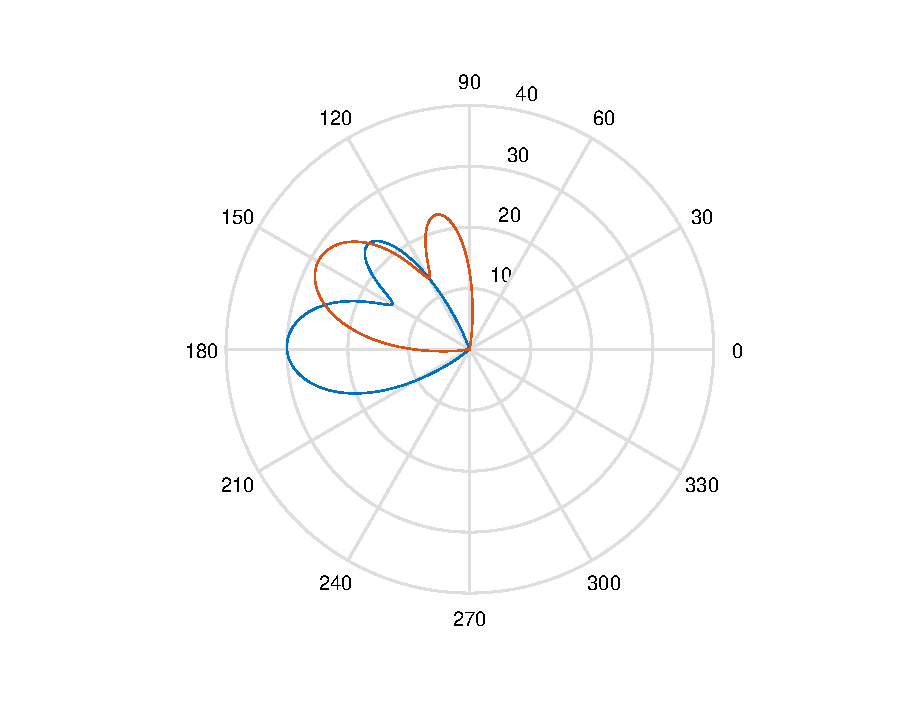
\includegraphics[width=10cm]{dirac_eff_pattern.eps}
  \caption{Resulting pattern for dirac impulses.}
  \label{fig:dirac_eff_pattern}
\end{figure}

The effect of a distribution instead of a simple dirac can be seen in \figref{fig:dist_eff_pattern}. The graph widens up and is blurred, which can be seen especially looking at the zeros. From this pattern, we can graphically determine the peak to null depth by evaluating the values at $\SI{90}{\degree}+\SI{90}{\degree}=\SI{180}{\degree}$ and $\SI{60.5}{\degree}+\SI{60.5}{\degree}=\SI{121}{\degree}$, which results in $\SI{15.13}{\decibel}$.


\begin{figure}[!h]
  \centering
  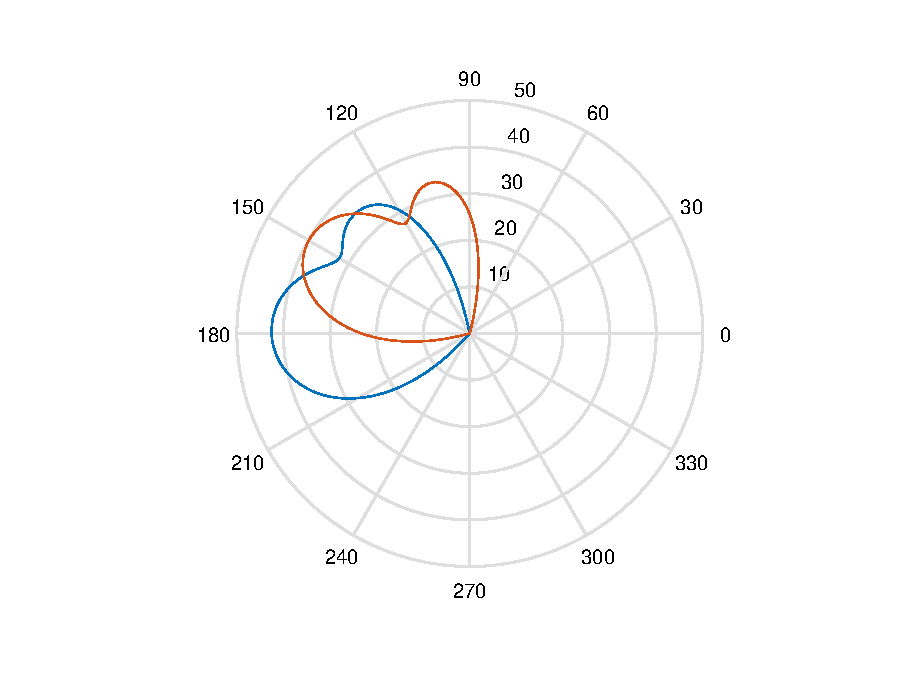
\includegraphics[width=10cm]{dist_eff_pattern.eps}
  \caption{Resulting pattern for the distributions.}
  \label{fig:dist_eff_pattern}
\end{figure}



\subsubsection{b) and c) What is the Cs/Is of the measured responses and what direction will the response function be centered at if performing a sweep (radar scan) with the antenna on the user and on the interferer?}

This value can be computed by two different methods. One is to integrate the product of the antenna pattern and the angular distribution of the users over the whole circle as shown in \equref{eq:bruteforce}.

\begin{flalign}
&&	\frac{Cs}{Is} =& \frac{\oint C(\varphi)\cdot a(\varphi)d\varphi}{\oint I(\varphi)\cdot a(\varphi)d\varphi}	 &\label{eq:bruteforce}
\end{flalign}

Another method to compute this result is to use the azimuthal measurement response of both, the user and the interferer. In \figref{fig:dist_eff_pattern}, the graph of the $m_{C}(\varphi)$ (blue) and $m_{I}(\varphi)$ (red) are shown.

Mathematically, performing a sweep (radar scan) is equivalent to find the correlation function described in \equref{eq:effective}. Due to the properties of this ``convolution'', the user (whose mean is located at 90 degrees) will be shifted $90 + 90$ degrees. As seen in \figref{fig:dist_eff_pattern}. The interferer, because of the same argument, will be shifted $60.5 + 60.5$ degrees.

In order to compute this result by this second method, we need to calculate the $Cs$ and the $Is$ using $m_{C}(\varphi)$ and $m_{I}(\varphi)$. This is done considering the user as a single source in $m_{C}(\varphi)$ at 180 degrees and the interferer as a single source in $m_{I}(\varphi)$ at 121 degrees. \textbf{MAYBE EXPAND THIS EXPLANATION}